\chapter{Epilogue: Final Adventures and Farewell}
\vspace{0.6cm}
\begin{center}
\nopagebreak
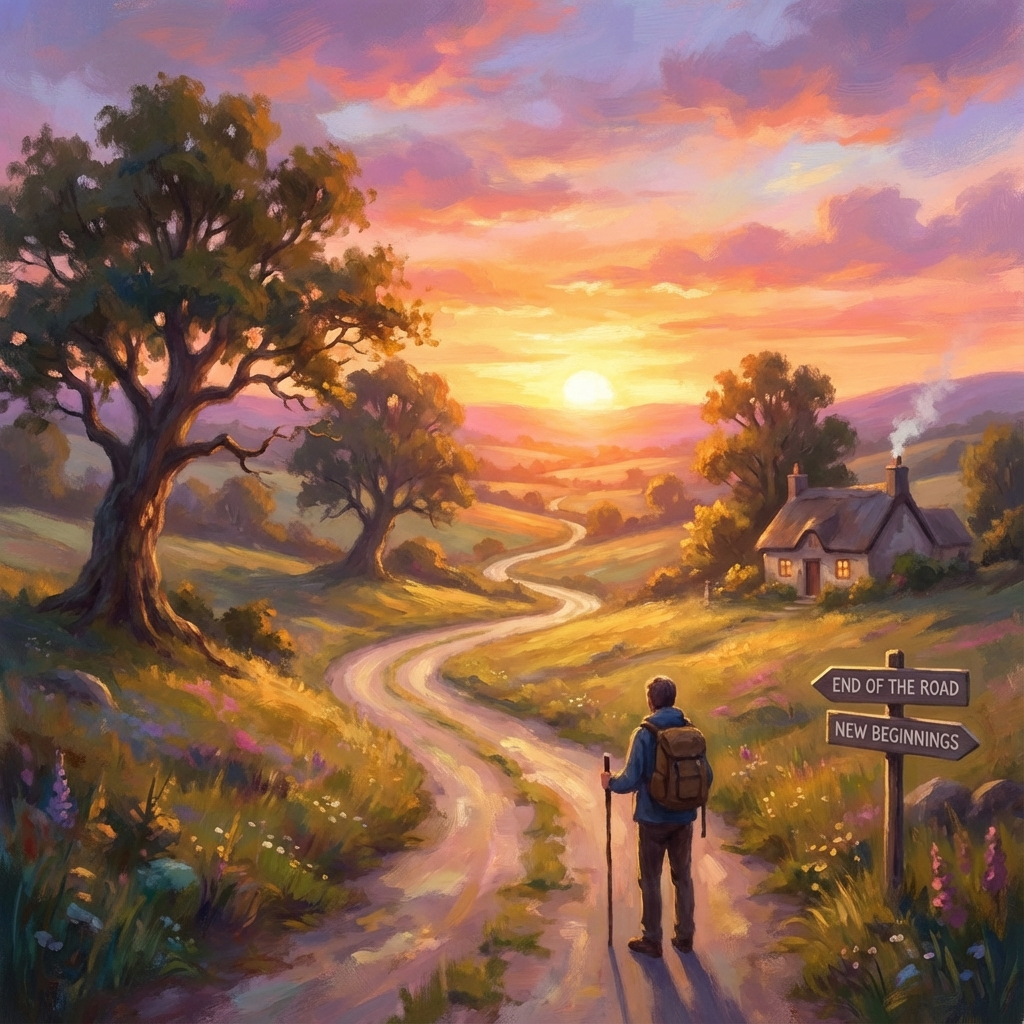
\includegraphics[width=0.75\textwidth,cfbox=gray!60 0.6pt 4pt]{sunset_road.png}\\
\vspace{4pt}
{\small\itshape Sunset on the road: the soul's journey continues.}
\end{center}

\vspace{0.6cm}
Jesus said goodbye to me at Atocha station. He was going to take a train, he said, to nowhere and everywhere.
—Will I see you again? —I asked, feeling a lump in my throat.


—You always see me —he smiled—. I am in the smile of the supermarket cashier. In the wind that moves the trees of Colmenarejo. In the silence of your room. But above all, I am in you. When you vibrate high, when you love, when you forgive... there I am. There we are one.


He gave me a big hug. He smelled like wood and fresh rain.
—Lead us not into temptation —he whispered in my ear—. Keep the frequency, friend. Keep the music playing. And if you ever get out of tune, don't judge yourself. Simply, tune in again.


He turned around and blended into the crowd. I watched him walk away, in his jeans and his quiet gait, among people running while looking at their phones. And for a moment, it seemed to me that the entire station lobby shone with a golden light.


I went out into the street. Madrid was still the same: noisy, chaotic, alive. But I was no longer the same. I took a deep breath, felt the sun on my face, and smiled. I was vibrating high. And I knew that, whatever happened, everything was going to be fine.


\textbf{The End.}